% Options for packages loaded elsewhere
\PassOptionsToPackage{unicode}{hyperref}
\PassOptionsToPackage{hyphens}{url}
%
\documentclass[
  ignorenonframetext,
  aspectratio=169]{beamer}
\usepackage{pgfpages}
\setbeamertemplate{caption}[numbered]
\setbeamertemplate{caption label separator}{: }
\setbeamercolor{caption name}{fg=normal text.fg}
\beamertemplatenavigationsymbolsempty
% Prevent slide breaks in the middle of a paragraph
\widowpenalties 1 10000
\raggedbottom
\setbeamertemplate{part page}{
  \centering
  \begin{beamercolorbox}[sep=16pt,center]{part title}
    \usebeamerfont{part title}\insertpart\par
  \end{beamercolorbox}
}
\setbeamertemplate{section page}{
  \centering
  \begin{beamercolorbox}[sep=12pt,center]{part title}
    \usebeamerfont{section title}\insertsection\par
  \end{beamercolorbox}
}
\setbeamertemplate{subsection page}{
  \centering
  \begin{beamercolorbox}[sep=8pt,center]{part title}
    \usebeamerfont{subsection title}\insertsubsection\par
  \end{beamercolorbox}
}
\AtBeginPart{
  \frame{\partpage}
}
\AtBeginSection{
  \ifbibliography
  \else
    \frame{\sectionpage}
  \fi
}
\AtBeginSubsection{
  \frame{\subsectionpage}
}
\usepackage{amsmath,amssymb}
\usepackage{iftex}
\ifPDFTeX
  \usepackage[T1]{fontenc}
  \usepackage[utf8]{inputenc}
  \usepackage{textcomp} % provide euro and other symbols
\else % if luatex or xetex
  \usepackage{unicode-math} % this also loads fontspec
  \defaultfontfeatures{Scale=MatchLowercase}
  \defaultfontfeatures[\rmfamily]{Ligatures=TeX,Scale=1}
\fi
\usepackage{lmodern}
\ifPDFTeX\else
  % xetex/luatex font selection
\fi
% Use upquote if available, for straight quotes in verbatim environments
\IfFileExists{upquote.sty}{\usepackage{upquote}}{}
\IfFileExists{microtype.sty}{% use microtype if available
  \usepackage[]{microtype}
  \UseMicrotypeSet[protrusion]{basicmath} % disable protrusion for tt fonts
}{}
\makeatletter
\@ifundefined{KOMAClassName}{% if non-KOMA class
  \IfFileExists{parskip.sty}{%
    \usepackage{parskip}
  }{% else
    \setlength{\parindent}{0pt}
    \setlength{\parskip}{6pt plus 2pt minus 1pt}}
}{% if KOMA class
  \KOMAoptions{parskip=half}}
\makeatother
\usepackage{xcolor}
\newif\ifbibliography
\setlength{\emergencystretch}{3em} % prevent overfull lines
\providecommand{\tightlist}{%
  \setlength{\itemsep}{0pt}\setlength{\parskip}{0pt}}
\setcounter{secnumdepth}{-\maxdimen} % remove section numbering
\PassOptionsToClass{aspectratio=169}{beamer}
\usepackage{../../../beamer_style/beamer_style}
\setbeamersize{text margin left=3.5mm,text margin right=3.5mm}
\ifLuaTeX
  \usepackage{selnolig}  % disable illegal ligatures
\fi
\usepackage{bookmark}
\IfFileExists{xurl.sty}{\usepackage{xurl}}{} % add URL line breaks if available
\urlstyle{same}
\hypersetup{
  pdftitle={Text Models for Measuring Ideology},
  pdfauthor={Jake S. Truscott, Ph.D},
  hidelinks,
  pdfcreator={LaTeX via pandoc}}

\title{Text Models for Measuring Ideology}
\subtitle{POS6933: Computational Social Science}
\author{Jake S. Truscott, Ph.D}
\date{}
\institute{\vspace{-5mm}

University of Florida \newline Spring 2026 \newline \newline \newline

\includegraphics[width=3cm]{../../../beamer_style/UF.png} \quad 

\includegraphics[width=3.1cm]{../../../images/CSS_POLS_UF_Logo.png}}

\begin{document}
\frame{\titlepage}

\section{Overview}\label{overview}

\begin{frame}{Overview}
\phantomsection\label{overview-1}
\begin{itemize}
\item Housekeeping
\item Class 9 Problem Set Review
\item \texttt{Wordscores}
\item \texttt{Wordfish}
\item \texttt{Wordshoal}
\item Office Hours (Until 6:00)
\end{itemize}
\end{frame}

\section{Housekeeping}\label{housekeeping}

\begin{frame}{Housekeeping}
\phantomsection\label{housekeeping-1}
\begin{itemize}
\item \textbf{Reminders}:
  \begin{itemize}
    \item Slides due to me and peer reviewers by 11:59pm on Sunday (Schedule \emph{Next}) \par \vspace{2.5mm}
    \item Final materials (Paper, Appendix, and Final Slides) due 4/24 (Canvas)  \par \vspace{2.5mm}
    \item Rubric \& help document located on Canvas (\textit{Files}) -- Be sure to follow formatting requirements...
  \end{itemize}
  \item I will stay until 6:00 today if you want to chat about your papers
\end{itemize}
\end{frame}

\begin{frame}{Housekeeping -- Presentation Order}
\phantomsection\label{housekeeping-presentation-order}
\centering
\scriptsize
\renewcommand{\arraystretch}{1.2}
\begin{tabular}{llll}
\hline
\textbf{Day} & \textbf{Student} & \textbf{Reviewer 1} & \textbf{Reviewer 2} \\
\hline
4/12 & Arora, Manya & Mamun & Revilla, Valeria \\
4/12 & Cui, Lixiao & Meneley, Cory & Sarver, Sarah \\
4/12 & Giron-Khalil, Jailyn & Mohammed, Suren & Sultana, Abida \\
4/12 & Hao, Tianshu & Oneil, Connor & Tierman, Hunter \\
4/12 & Islam, Md Sahidul & Revilla, Valeria & Trenchi, Alejandro \\
4/12 & Mamun & Sarver, Sarah & Wang, Qianxi \\
4/12 & Meneley, Cory & Sultana, Abida & Arora, Manya \\
4/12 & Mohammed, Suren & Tierman, Hunter & Cui, Lixiao \\
4/19 & Oneil, Connor & Trenchi, Alejandro & Giron-Khalil, Jailyn \\
4/19 & Revilla, Valeria & Wang, Qianxi & Hao, Tianshu \\
4/19 & Sarver, Sarah & Arora, Manya & Islam, Md Sahidul \\
4/19 & Sultana, Abida & Cui, Lixiao & Mamun \\
4/19 & Tierman, Hunter & Giron-Khalil, Jailyn & Meneley, Cory \\
4/19 & Trenchi, Alejandro & Hao, Tianshu & Mohammed, Suren \\
4/19 & Wang, Qianxi & Islam, Md Sahidul & Oneil, Connor \\
\hline
\end{tabular}
\end{frame}

\begin{frame}{Class 9 Problem Set Review}
\phantomsection\label{class-9-problem-set-review}
\begin{itemize}
\item Notes...
\end{itemize}
\end{frame}

\section{Text Models for Ideology}\label{text-models-for-ideology}

\begin{frame}{Scaling Ideology}
\phantomsection\label{scaling-ideology}
\end{frame}

\begin{frame}{Scaling Ideology (Cont.)}
\phantomsection\label{scaling-ideology-cont.}
\begin{itemize}
\item \textbf{How I Was Taught to Think of It}: Rather than using right-hand side of the equation to solve for the left, flip the intuition -- Use DV to estimate optimal IV(s). \par \vspace{2.5mm} \pause
\item Assumptions: 
  \begin{enumerate}
  \item \textbf{Stable Latent Preferences}: Assumes actors have stable, coherent, underlying ideological positions that guide their behavior. \par \vspace{2.5mm} \pause
  \item \textbf{Behavior Reflects Ideology}: Treats votes or language as meaningful signals of those latent preferences (not pure noise or strategy). \par \vspace{2.5mm} \pause
  \item \textbf{Common Dimensional Structure}: Assumes actors operate in a shared ideological space (often low-dimensional) that is comparable across observations. 
  \end{enumerate}
\end{itemize}
\end{frame}

\begin{frame}{Scaling Ideology (Goals)}
\phantomsection\label{scaling-ideology-goals}
\begin{itemize}
\item \textbf{Recover Latent Position(s)}: Using observable behaviors as signals (ex: votes on legislation), estimate an underlying ideological dimension that isn't directly observed but we know exists and can be represented given both directionality (e.g., \emph{Left-Right}) and magnitude (e.g., \emph{Very Left}-\emph{Very Right}). \par \vspace{2.5mm} \pause
\item \textbf{Place Actors (Groups) On a Spectrum}: Relative location of actors (groups) in a common space denotes cardinality (and proximity) of relationship in that dimension.
\end{itemize}
\end{frame}

\begin{frame}{Text Models for Ideology (Benefits)}
\phantomsection\label{text-models-for-ideology-benefits}
\begin{itemize}
\item Binary votes sometimes insufficient to fully understand elite political behaviors \par \vspace{2.5mm}
\item Text leverages high dimensional structure -- more variance and perhaps better explanatory power.  \par \vspace{2.5mm}
\item Text captures nuance in reasoning, framing, and emphasis that votes alone cannot reveal \par \vspace{2.5mm}
\item Enables dynamic and context-sensitive measurement of ideology across issues, time, and audiences
\end{itemize}
\end{frame}

\begin{frame}{Models Today}
\phantomsection\label{models-today}
\begin{itemize}
\item Going to focus on 3 models: \texttt{Wordscores, Wordfish}, and \texttt{Wordshoal} \par \vspace{2.5mm}
\item \textbf{Important}: View subsequent models as methodological improvements on preceding \par \vspace{2.5mm}
\end{itemize}
\end{frame}

\section{Wordscores}\label{wordscores}

\begin{frame}{Wordscores (Laver, Benoit, and Garry)}
\phantomsection\label{wordscores-laver-benoit-and-garry}
\begin{itemize}
\item Developed by Laver, Benoit, and Garry (2003) -- Probably not(?) first text-based model of ideology, but certainly first to gain significant use in social sciences. \par \vspace{2.5mm}
\item It’s effectively (sort of) Naive Bayes + Value Projection onto a Reference Scale + Rescaling \par \vspace{2.5mm} \pause 
\item \textit{Recall...} for standard Naive Bayes, we: 
\begin{enumerate}
  \item Estimate how likely each word $w$ is to appear in each class $k$ -- $p(w\mid k)$ \pause
  \item For new document $D_{i}$, we use those learned word probabilities to calculate $\pi_{ik}$ (probability that $D_{i}$ belongs in each possible class -- $p(k|mid D_i)$ \pause
  \item Classification assigned to the document because it has the highest probability
\end{enumerate}
\end{itemize}
\end{frame}

\begin{frame}{Wordscores (Laver, Benoit, and Garry) -- Cont.}
\phantomsection\label{wordscores-laver-benoit-and-garry-cont.}
\begin{itemize}
  \item \textbf{What \texttt{Wordscores} does instead}: Estimate how likely it is that each word belongs to a reference document -- $p(w\mid r)$, where $A_{r}$ represents the ideological score of those reference documents. \par \vspace{2.5mm} \pause 
  \item $ S_{w} = \sum_{r}p(r\mid w)A_{r} $ --  the score of some word $S_{w}$ is the sum of the probabilities it belongs to each reference document times the score associated with those documents. \par \vspace{2.5mm} \pause
  \item New documents $v$ are finally rescaled to account for weighted averages of word scores -- such that a document's position is the average ideology of the words it uses (from the reference documents) and weighted by the word frequences: 
  \item[] $$ S_{v} = \sum_{w}p(w\mid v)S_{w} $$
\end{itemize}
\end{frame}

\begin{frame}{Wordscores Example}
\phantomsection\label{wordscores-example}
\begin{columns}[T]
    \begin{column}{0.4\textwidth}
    \centering
    \begin{tabular}{lccc}
    \toprule
    Word & Left Ref. & Right Ref. & TOTAL \\
    \midrule
    welfare & 8 & 1 & 9 \\
    tax & 2 & 6 & 8 \\
    military & 1 & 7 & 8 \\
    \midrule
    \textbf{TOTAL} & 11 & 14 & 25 \\
    \bottomrule
    \end{tabular}
    \end{column}
    \begin{column}{0.6\textwidth}
    \begin{itemize}
        \item 3 Words (\emph{welfare, tax, military}) \par \vspace{2.5mm}
        \item 2 reference documents: 
        \begin{itemize}
          \item[] $A_{Left} = (-1)$ 
          \item[] $A_{Right} = (+1)$
        \end{itemize}
    \end{itemize}
    \end{column}
\end{columns}
\end{frame}

\begin{frame}{Wordscores Example (Cont.)}
\phantomsection\label{wordscores-example-cont.}
\begin{columns}[T]
    \begin{column}{0.4\textwidth}
    \centering
    \footnotesize
    \begin{tabular}{lccc}
    \toprule
    Word & Left Ref. & Right Ref. & TOTAL \\
    \midrule
    welfare & 8 & 1 & 9 \\
    tax & 2 & 6 & 8 \\
    military & 1 & 7 & 8 \\
    \midrule
    \textbf{TOTAL} & 11 & 14 & 25 \\
    \bottomrule
    \end{tabular}
    \end{column}
    \begin{column}{0.6\textwidth}
    \normalsize
    \begin{itemize}
        \item Let's start with word probabilities: 
        \item[] $p(\text{left}\mid \text{welfare}) = \frac{8}{9} = 0.889$ 
        \item[] $p(\text{right}\mid \text{welfare}) = \frac{1}{9} = 0.111$ \pause 
        \item[] $p(\text{left}\mid \text{tax}) =$ \pause $\frac{2}{8} = 0.25$ 
        \item[] $p(\text{right}\mid \text{tax}) =$ \pause $\frac{2}{8} = 0.75$
        \item[] $p(\text{left}\mid \text{military}) =$ \pause $\frac{1}{8} = 0.125$
        \item[] $p(\text{right}\mid \text{military}) =$ \pause $\frac{7}{8} = 0.875 $
    \end{itemize}
    \end{column}
\end{columns}
\end{frame}

\begin{frame}{Wordscores Example (Cont.)}
\phantomsection\label{wordscores-example-cont.-1}
\begin{columns}[T]
    \footnotesize
    \begin{column}{0.4\textwidth}
    \centering
    \begin{tabular}{lcc}
    \toprule
    Word & $p(\text{left}\mid w)$ & $p(\text{right}\mid w)$ \\
    \midrule
    welfare & 0.889 & 0.111 \\
    tax & 0.25 & 0.75 \\
    military & 0.125 & 0.875 \\
    \bottomrule
    \end{tabular}
    \end{column}
    \begin{column}{0.6\textwidth}
    \normalsize
    \begin{itemize}
        \item Now we can compute the word scores using 
        $S_{w} = \sum_{r}p(r\mid w)A_{r}$: \par \vspace{5mm}
        \item[] $S_{\text{welfare}} = 0.889(-1_{Neg}) + 0.111(1_{Pos}) = -0.778$ \par \vspace{2.5mm}
        \item[] $S_{\text{tax}}$ \pause $= 0.25(-1_{Neg}) + 0.75(1_{Pos}) = 0.50$ \par \vspace{2.5mm}
        \item[] $S_{\text{military}}$ \pause $= 0.125(-1_{Neg}) + 0.875(1_{Pos}) = 0.75$ 
    \end{itemize}
    \end{column}
\end{columns}
\end{frame}

\begin{frame}{Wordscores Example (Cont.)}
\phantomsection\label{wordscores-example-cont.-2}
\begin{itemize}
\item We can now start computing document scores for new documents $S_{v} = \sum_{w}p(w\mid v)S_{w}$ \par \vspace{2.5mm}
\item  Suppose a new document ($S_{v}$) contains the following: \textbf{Welfare} (3), \textbf{Tax} (1), and  \textbf{Military} (0).\par \vspace{2.5mm} 
\item We know that $p(\text{welfare}\mid v) = \frac{3}{4} = 0.75$, and $p(\text{tax}\mid v) = \frac{1}{4} = 0.25$. \par \vspace{2.5mm}
\item Solve for $S_{v}$ \pause $ = 0.75(-0.778) + 0.25(0.5) = (-0.458)$
\end{itemize}
\end{frame}

\begin{frame}{Wordscores Example (Cont.)}
\phantomsection\label{wordscores-example-cont.-3}
\begin{center}
\includegraphics{class_10_text_models_ideology_files/figure-beamer/visualizing_wordscores-1} \end{center}
\end{frame}

\begin{frame}{Wordscores Example (Cont.)}
\phantomsection\label{wordscores-example-cont.-4}
\begin{itemize}
\item Recall: $S_{v} = \sum_{w}p(w\mid v)S_{w}$ \par \vspace{2.5mm}
\item  Suppose another new document ($S_{v}$) contains the following: \textbf{Welfare} (2), \textbf{Tax} (5), and  \textbf{Military} (3).\par \vspace{2.5mm} 
\item $p(\text{Welfare}\mid v) = 0.20$, $p(\text{Tax}\mid v) = 0.5$, and $p(\text{Military}\mid v) = 0.33$
\item Solve for $S_{v}$ \pause $ = 0.20(-0.778) + 0.5(0.25) + 0.33(0.75) = 0.217$ 
\end{itemize}
\end{frame}

\begin{frame}{Wordscores Example (Cont.)}
\phantomsection\label{wordscores-example-cont.-5}
\begin{center}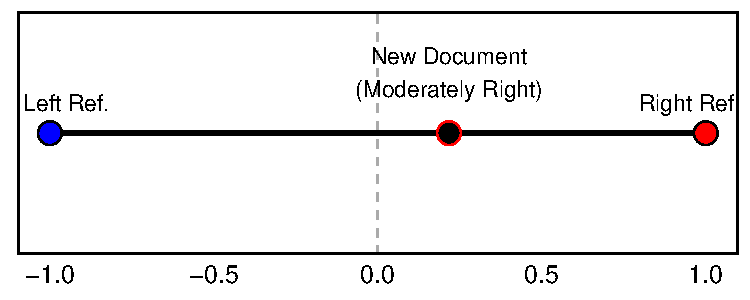
\includegraphics{class_10_text_models_ideology_files/figure-beamer/visualizing_wordscores_2-1} \end{center}
\end{frame}

\section{Wordfish}\label{wordfish}

\begin{frame}{Wordfish (Slapin and Proksch)}
\phantomsection\label{wordfish-slapin-and-proksch}
\begin{itemize}
\item \texttt{Wordfish} is a poisson factor model that (like Wordscores) tries to scale the ideological positions of documents. \par \vspace{2.5mm}  \pause 
\item It does \textbf{not} require reference documents -- it is \textbf{unsupervised} \par \vspace{2.5mm} 
\item Uses maximum likelihood to infer both a document's latent position $\theta_i$ and word discrimination $\beta_j$ (how strongly a word separates documents) \par \vspace{2.5mm} 
\item[] 
\end{itemize}
\end{frame}

\begin{frame}{Wordfish Specification}
\phantomsection\label{wordfish-specification}
\begin{itemize}
\item[] $$x_{ij} \sim \text{Poisson}(\lambda_{ij})$$
\item[]  $$\lambda_{ij} = \exp(\alpha_{j} + \psi_j + \beta_j\theta_i) $$
\item[] Where: 
\footnotesize
  \begin{itemize}
  \item $x_{ij}$ = the count of word $j$ in document $i$ 
\item $\alpha_{i}$ = Document-specific verbosity (value to control for length of document -- ensures $\theta_i$ reflects content differences, not just document size) 
\item $\phi_j$ = Word-specific baseline frequency 
\item $\beta_j$ = Word-specific discrimination 
\item $\theta_i$ = Latent position of document $i$ (\textbf{What we're most interested in}!)
  \end{itemize}
\end{itemize}
\end{frame}

\end{document}
